    \subsection*{The Optimal Direction: The Gradient}
    
        How do we get the optimal direction?
        
        The \textbf{total} change in $J$ is gotten by just \textbf{adding} the change in each direction (thank you planes!):
        
        \begin{figure}[H]
        
                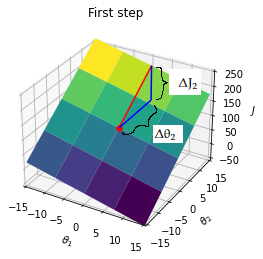
\includegraphics[width=70mm,scale=0.5]{images/gradient_descent_images/first_step.png}
                
                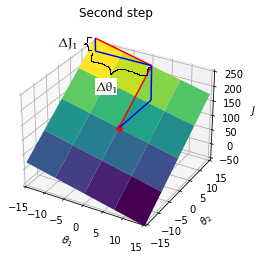
\includegraphics[width=70mm,scale=0.5]{images/gradient_descent_images/second_step.png}
                
            \caption*{You can add up the results of our two steps: $\Delta J_2$ and $\Delta J_1$.}
        \end{figure}
        
        \begin{equation}
            \Delta J \approx \Delta J_1 + \Delta J_2
        \end{equation}
        
        Let's convert that using derivatives:
        
        \begin{equation}
            \Delta J \approx
            \Delta \theta_1 \pderiv{J}{\theta_1} +
            \Delta \theta_2 \pderiv{J}{\theta_2}
        \end{equation}
        
        Now we've got a useful equation: the total change. As a bonus we can see a clear \textbf{pattern} ($\nth{i}$ $\theta$ matches $\nth{i}$ derivative). 
        
        So, \textbf{condense} this pattern, like we did for our linear model: using a \textbf{dot product}.
        
        \begin{equation}
            \Delta J 
            \approx 
            \begin{bmatrix}
              \Delta \theta_1 \\ \Delta \theta_2
            \end{bmatrix}
            \cdot
            \begin{bmatrix}
                \pderivslash{J}{ \theta_1}  \\ 
                \pderivslash{J}{ \theta_2 } 
            \end{bmatrix}
            =
            \Delta \theta \cdot \nabla_\theta J
        \end{equation}
        
        The \textbf{gradient} shows up! Interesting. But what does that \textbf{mean}?
        
        Well, we want to \textbf{maximize} (or minimize!) our $\Delta J$. How do we maximize a \textbf{dot product}?
        
        By making sure the directions are \textbf{the same}! So, we can confirm that the \textbf{gradient} gives us the \textbf{best} direction.
        
        So, all we have to do is to \textbf{flip} the sign to \textbf{minimize} $\Delta J$.
            \note{And so, gradient descent is already complete!}\\
        
        \begin{concept}
            The \vocab{gradient} $\nabla J$ is the \vocab{direction of greatest increase} for $J$.
            
            That means means the opposite direction $-\nabla J$ is the \vocab{direction of greatest decrease} in $J$.
        \end{concept}
        
        This is the single \textbf{most important concept} in this entire chapter!
        